\documentclass{article}
\usepackage[a4paper, margin=2cm]{geometry}

\usepackage{amsmath}
\usepackage{amssymb}
\usepackage{mathtools}
\usepackage{amstext}
\usepackage{amsthm}
\usepackage{fancyhdr}
\usepackage{siunitx}
\usepackage{physics}

\usepackage{hyperref}


\usepackage{graphicx}
\usepackage{float}
\graphicspath{{figures/}} %Setting the graphicspath
\usepackage{float}
\usepackage{caption}
\usepackage{subcaption}

%% To work with inkfigures
%\usepackage{import}
%\usepackage{pdfpages}
%\usepackage{transparent}
%\usepackage{xcolor}

\newcommand{\incfig}[2][1]{%
    \def\svgwidth{#1\columnwidth}
    \import{./figures/}{#2.pdf_tex}
}

\pdfsuppresswarningpagegroup=1

%\graphicspath{{figures/}}

\pagestyle{fancy}
\rhead{Alexandre Adam}
\lhead{PHY6669 -- Cosmologie \\ Alan Robinson}
\chead{Devoir 3}
\rfoot{\today}
\cfoot{\thepage}

\newcommand{\angstrom}{\textup{\AA}}
\numberwithin{equation}{section}
\renewcommand\thesubsection{\alph{subsection})}
\renewcommand\thesubsubsection{\Roman{subsubsection}}
\newcommand{\s}{\hspace{0.1cm}}

\newcommand{\pyoutput}[2]{#2}

% Astronomy
\DeclareSIUnit\parsec{pc}
\DeclareSIUnit\lightyear{ly}

\begin{document}
\section{Nucléosynthèse}
\subsection{Dodelson ch. 3, Exercice 2}
La densité numérique des électrons-positrons est donnée en terme de la distribution 
de Fermi-Dirac (on conserve les constantes physiques $c,\, \hbar,\, k_B$ pour ce 
sous-numéro):
\begin{equation}\label{eq:nelectron} 
        n_{e^\pm}^{(0)} = g_{e^\pm}\int \frac{d^3p}{(2 \pi \hbar)^{3}} 
        \frac{1}{\exp \left\{ \dfrac{E(p)}{k_B T} \right\} + 1}
\end{equation} 
où $E(p) = \sqrt{p^2 c^2 + m_e^2c^4}$ et $g_{e^\pm} = 2$ pour les états de spins. 
On a négligé le potentiel chimique des électrons $\mu_e$ car il est 
identiquement nul avant et durant la nucléosynthèse.
%dû à notre supposition que 
%le processus $e^- + e^+ \longleftrightarrow \gamma + \gamma$ est à l'équilibre.
À la 
température où la nucléosynthèse se produit ($k_BT \simeq 1\, \text{MeV}$), on ne 
peut pas simplifier l'énergie en faveur de $p$ ou $m_e$ puisque la masse de l'électron
$m_e \simeq 0.5\, \text{MeV}/c^2$ est similaire à la température. 
\begin{figure}[H]
        \centering
        \begin{subfigure}[t]{0.45\textwidth}
                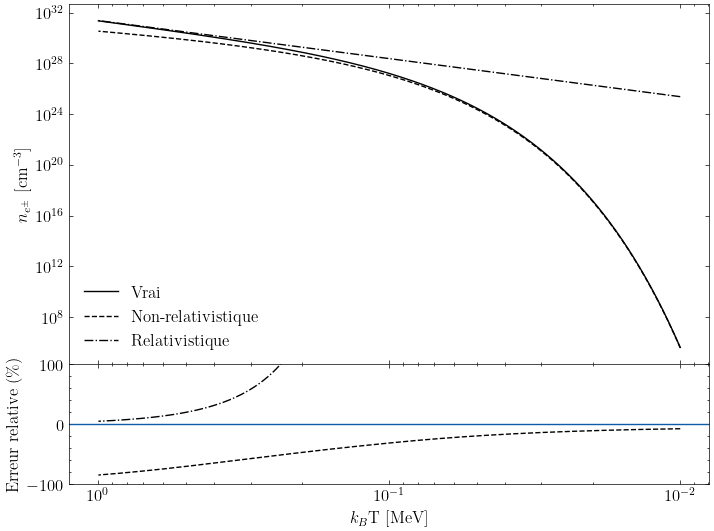
\includegraphics[width=\textwidth]{nucleosynthesis_electron_density}
                \caption{Comparaison des approximations à la vrai fonction durant l'époque de 
                nucléosynthèse.}
                \label{fig:Comparaison}
        \end{subfigure}
        ~
        \begin{subfigure}[t]{0.45\textwidth}
                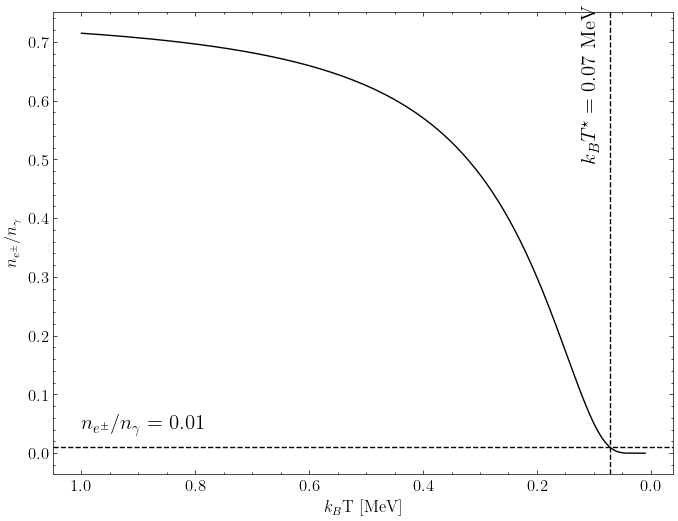
\includegraphics[width=\textwidth]{resultat_ratio_ne_ngamma}
                \caption{Ratio des densités numérique des électrons-positrons 
                lors de l'époque de nucléosynthèse.}
                \label{fig:Res1}
        \end{subfigure}
\end{figure}
La densité numérique des photons se calcule directment à partir de la distribution 
de Planck
\begin{equation}\label{eq:PlanckDensity} 
        n_\gamma^{(0)} = g_\gamma\int_0^{\infty}4\pi\frac{B(\nu, T) d\nu}{h\nu} = 
        \frac{8 \pi }{c^3}  \int_0^{\infty } 
        \frac{\nu^2 d\nu}{\exp \left\{ h\nu / k_B T \right\} - 1}
\end{equation} 
Avec substition on retrouve une forme standard pour l'intégrale qui devient
\[
        n_\gamma^{(0)} = \frac{2\zeta(3 )}{\pi^2} \left( \frac{k_B T}{\hbar c} \right)^{3}
\]
où $\zeta(s)$ est la fonction zeta de Riemann.
On cherche la température $T^\star$ à partir de laquelle la densité numérique des électrons 
devient $1\%$ celle des photons $n_\gamma^{(0)}$. En interpolant une grille de valeurs, 
on obtient
\[
        \boxed{k_BT^\star = 0.06\, \text{MeV}}
\]

Avec un ratio de baryons sur photons de
\[
        \eta_b = 6 \times 10^{-10}
\]
au moment de la nucléosynthèse (après annihilation des anti-particules), on peut 
tenter de déterminer le moment (la température) à partir duquel les électrons 
ne seront plus en équilibre avec le processus de création/annihiltion de paires. En 
effet, l'Univers observé est électriquement neutre et on doit avoir $n_{e^{-}} = n_p$ 
à un certains moment. Si on suppose que la grande majorité de la matière baryonique 
est constitué de protons (on néglige les neutrons), alors on trouve
\[
        \boxed{k_B T( \frac{n_{e^{-}}}{n_\gamma} \sim \eta_b) \simeq 0.02\, \text{MeV}}
\]

\subsection{Dodelson ch. 3, Exercice 3}
\subsubsection{Intégrale sur les particules massives}
On cherche à calculer le taux de la conversion de neutrons en protons $\Gamma_{np}$.
Pour ce faire, on estime la section efficace thermal des processus 
$n + \nu_e \longrightarrow p + e^{-}$ et $n + e^{+} \longrightarrow p + \bar{\nu}_e$. 
On néglige la masse de l'électron et on assume que les processus peuvent être 
décrits pas les statistiques de Boltzmann. Dans quel cas leur taux de réaction 
est le même. On considère un seul processus pour le moment et on néglige les 
facteurs de Pauli ($f_i \ll 1$):
\begin{align*}
        \expval{\sigma v} &\equiv \frac{1}{n_n^{(0)} n_{e^{+}}^{(0)}}
        \int \frac{d^{3}\mathbf{p}_n}{(2\pi)^{3}2E_{n}}
        \int \frac{d^{3}\mathbf{p}_{e^{+}}}{(2\pi)^{3}2E_{e^{+}}}
        \int \frac{d^{3}\mathbf{p}_{p}}{(2\pi)^{3}2E_p}
        \int \frac{d^{3}\mathbf{p}_{\bar{\nu}_e}}{(2\pi)^{3}2E_{\bar{\nu}_e}}
        \exp \left\{ - \frac{E_{p_n} + E_{p_{e^{+}}}}{T} \right\}\\
                          &\s\s\s\s\times 
        (2 \pi)^{4} \delta^{(3)}(\mathbf{p}_n + 
        \mathbf{p}_{e^{+}} - \mathbf{p}_p - \mathbf{p}_{\bar{\nu}_e}) 
        \delta(E_{n} + E_{e^{+}} - E_p - E_{\bar{\nu}_e})
        |\mathcal{M}|^{2}
\end{align*}
En négligeant la masse des neutrinos (ce qui est toujours valide) et la masse des 
électrons (valide devant la masse du protons et du neutrons $m_p \sim m_n \sim 2000m_e$), 
alors $E_{e^{+}} = p_{e^{+}} = |\mathbf{p}_{e^{+}}|$ et 
$E_{\bar{\nu}_e} = p_{\bar{\nu}_e}$. De plus,
on approxime l'énergie des particules massive par leur énergie de masse 
$E_p \simeq m_p$ et $E_n \simeq m_n$ ce qui est valide durant la 
nucléosynthèse puisque la température est de $\sim1\, \text{MeV} \ll m_p$.
%Aussi, on peut utiliser la fonction $\delta$ pour remplacer $p_n$ par 
%$p_{\bar{\nu}_e}$ et $p_p$ par $p_{e^{+}}$, ce qui 
%nous laisse
\begin{align*}
        \expval{\sigma v} &= \frac{1}{n_n^{(0)} n_{e^{+}}^{(0)}}
        \int \frac{d^{3}\mathbf{p}_n}{(2\pi)^{3}2m_n}
        \int \frac{d^{3}\mathbf{p}_{e^{+}}}{(2\pi)^{3}2p_{e^{+}}}
        \int \frac{d^{3}\mathbf{p}_{p}}{(2\pi)^{3}2m_p}
        \int \frac{d^{3}\mathbf{p}_{\bar{\nu}_e}}{(2\pi)^{3}2p_{\bar{\nu}_e}}
        \exp \left\{ - \frac{m_n + p_{e^{+}}}{T} \right\}\\
                          &\s\s\s\s\times 
        (2 \pi)^{4 } \delta^{(3)}(\mathbf{p}_n + 
        \mathbf{p}_{e^{+}} - \mathbf{p}_p - \mathbf{p}_{\bar{\nu}_e}) 
        \delta(\mathcal{Q} + p_{e^{+}} - p_{\bar{\nu}_e})
        |\mathcal{M}|^{2}
\end{align*}
où on a définit $\mathcal{Q} = m_n - m_p = 1.293\, \text{MeV}$. On fait l'intégrale 
sur l'espace de phase des particules massives sur une coquille dans 
le système de référence du neutron (le choix est libre puisque 
l'intégrale est un invariant de Lorentz), de sortes que $\mathbf{p}_n = 0$. 
La fonction $\delta $ de Dirac restante sélectionne alors 
$\mathbf{p}_{e^{+}} = \mathbf{p}_p + \mathbf{p}_{\bar{\nu}_e}$ par 
conservation de la quantité de mouvement et on obtient (en appliquant 
la fonction $\delta^{3}$ sur $\int d^{3}\mathbf{p}_p$):

\begin{align*}
        \expval{\sigma v} &= \frac{1}{n_n^{(0)} n_{e^{+}}^{(0)}}
        \frac{2\pi}{ 4m_n m_p}
        \int \frac{d^{3}\mathbf{p}_n}{(2\pi)^{3}}
        \int \frac{d^{3}\mathbf{p}_{e^{+}}}{(2\pi)^{3}2p_{e^{+}}}
        \int \frac{d^{3}\mathbf{p}_{\bar{\nu}_e}}{(2\pi)^{3}2p_{\bar{\nu}_e}}
        \exp \left\{ - \frac{m_n + p_{e^{+}}}{T} \right\}\\
                          &\s\s\s\s\times 
        \delta(\mathcal{Q} + p_{e^{+}} - p_{\bar{\nu}_e})
        |\mathcal{M}|^{2}
\end{align*}
À l'équilibre, 
\[
        n_n^{(0)} = 2\int \frac{d^{3}\mathbf{p}_n}{(2\pi)^{3}}\exp \left\{ -\frac{m_n}{T} \right\}
\]
De sortes que 
\begin{align*}
        \Aboxed{\expval{\sigma v} &= \frac{1}{n_{e^{+}}^{(0)}}
        \frac{\pi}{ 4m_n m_p}
        \int \frac{d^{3}\mathbf{p}_{e^{+}}}{(2\pi)^{3}2p_{e^{+}}}
        \int \frac{d^{3}\mathbf{p}_{\bar{\nu}_e}}{(2\pi)^{3}2p_{\bar{\nu}_e}}
        \exp \left\{ - \frac{p_{e^{+}}}{T} \right\}
        \delta(\mathcal{Q} + p_{e^{+}} - p_{\bar{\nu}_e})
|\mathcal{M}|^{2}}
\end{align*}


\subsubsection{Taux de réaction}
L'amplitude de la réaction est
\begin{equation}\label{eq:AmpReaction} 
        |\mathcal{M}|^{2} = 32 G_F^2(1 + 3g_A^2)m_p^2p_{\nu}p_e
\end{equation} 
où $g_A$ est le vecteur axial de couplage du nucléon qu'on mesure 
aujourd'hui via le temps de vie du neutron
\[
        \tau_n^{-1} = \lambda_0G_F^2(1 + 3g_A^2) \frac{m_e^5}{2\pi^3}
\]
où $\lambda_0 \simeq 1.636$, $\tau_n = 879.4 \pm 0.6\,\, \text{s}$ et 
$G_F$ est la constante de Fermi
\[
        G_F = 1.16639(1) \times 10^{-5}\, \text{GeV}^{-2} (\hbar c)^{3}
\]
On performe 
l'intégrale de la section efficace thermalisée sur une 
coquille dans l'espace de phase du positron. On applique en 
premier lieu la fonction $\delta $ sur l'énergie:
\begingroup
\allowdisplaybreaks
\begin{align*}
        n_{e^{+}}^{(0)}\expval{\sigma v} &= 
        \frac{32\pi G_F^2(1 + 3g_A^2) m_p}{ 4m_n}
        \int \frac{d^{3}\mathbf{p}_{e^{+}}}{(2\pi)^{3}2p_{e^{+}}}
        \int \frac{d^{3}\mathbf{p}_{\bar{\nu}_e}}{(2\pi)^{3}2p_{\bar{\nu}_e}}
        \exp \left\{ - \frac{p_{e^{+}}}{T} \right\}
        \delta(\mathcal{Q} + p_{e^{+}} - p_{\bar{\nu}_e})
        p_{\bar{\nu}_e} p_{e^{+}} \\
        &= 
        \frac{32\pi G_F^2(1 + 3g_A^2) m_p}{ 4m_n}
        \int_0^{\infty } \frac{4 \pi p^2_{e^{+}} dp_{e^{+}}}{(2\pi)^{3}2p_{e^{+}}}
        \int_0^{\infty } \frac{4 \pi p^2_{\bar{\nu}_e} dp_{\bar{\nu}_e}}{(2\pi)^{3}2p_{\bar{\nu}_e}}
        \exp \left\{ - \frac{p_{e^{+}}}{T} \right\}
        \delta(\mathcal{Q} + p_{e^{+}} - p_{\bar{\nu}_e})
        p_{\bar{\nu}_e} p_{e^{+}} \\
        &= 
        \frac{4 G_F^2(1 + 3g_A^2) m_p}{ (2\pi)^{3}m_n}
        \int_0^{\infty }  p^2_{e^{+}} dp_{e^{+}}
        \int_0^{\infty }  p^2_{\bar{\nu}_e} dp_{\bar{\nu}_e}
        \exp \left\{ - \frac{p_{e^{+}}}{T} \right\}
        \delta(\mathcal{Q} + p_{e^{+}} - p_{\bar{\nu}_e})
        \\
        &= 
        \frac{4 G_F^2(1 + 3g_A^2) m_p}{ (2\pi)^{3}m_n}
        \int_0^{\infty }  dp_{e^{+}} p^2_{e^{+}} 
        (\mathcal{Q} + p_{e^{+}})^2
        \exp \left\{ - \frac{p_{e^{+}}}{T} \right\}
\end{align*}
\endgroup
On applique la substitution $y \equiv \dfrac{p_{e^{+}}}{T}$ pour obtenir
\begin{align*}
        n_{e^{+}}^{(0)}\expval{\sigma v} &= 
        \frac{4 G_F^2(1 + 3g_A^2) m_p}{ (2\pi)^{3}m_n}T^3
        \int_0^{\infty }  dy\,\, y^2  (\mathcal{Q}^2 + 2\mathcal{Q}Ty + T^2y^2)
        e^{-y}
\end{align*}
On reconnaît la forme intégrale de la fonction $\Gamma(s)$, ainsi
\begin{align*}
        n_{e^{+}}^{(0)}\expval{\sigma v} &= 
        \frac{4 G_F^2(1 + 3g_A^2) m_p}{ (2\pi)^{3}m_n}T^3
        \left[\Gamma(3) \mathcal{Q}^{2} + 2\Gamma(4) \mathcal{Q}T
        + \Gamma(5)T^2 \right] \\
        &= 
        \frac{4 G_F^2(1 + 3g_A^2) m_p}{ (2\pi)^{3}m_n}T^3
        \left[ 2\mathcal{Q}^{2} + 12 \mathcal{Q}T
        + 24T^2 \right] \\
        &= 
        \frac{16 \pi^3 m_p}{ \lambda_0(2\pi)^{3}\tau_n m_e^5 m_n}T^3
        \left[ \mathcal{Q}^{2} + 6 \mathcal{Q}T
        + 12T^2 \right] \\
\end{align*}
%Avec les valeurs numériques mentionnées plus haut, on trouve le facteur lié au 
%vecteur de couplage axial:
%\[
        %\boxed{ 1 + 3g_A^2 = 23.9}
%\]
En posant de plus $x \equiv \dfrac{\mathcal{Q}}{T}$, on trouve
\[
        \boxed{\Gamma_{np} = 2 n_{e^{+}}^{(0)} \expval{\sigma v} 
        = 
        \frac{ 4 m_p \mathcal{Q}^5}{ \lambda_0 \tau_n m_e^5 m_n} \frac{1}{x^5}
        \left[ x^2 + 6x 
+ 12 \right]}
\]
On peut comparer avec l'équation (3.29) et on remarque qu'on 
obtient
\[
        \boxed{\Gamma_{np} \simeq \frac{253.57}{\tau_n x^5} \left[ x^2 + 6x + 12 \right]}
\]
La constante numérique $253$ est comparable à $255$, 
celle obtenue par Bernstein (1988).
%\citet{Bernstein1988}.

\section{Vitesse du son lors du découplement}


\subsection{Ratio de densité}
On cherche 
\[
        R \equiv \frac{3\rho_b}{4\rho_\gamma}
\]
où l'indice $b$ réfère aux baryons.

La première loi de la thermodynamique avec $dQ=0$ 
dans un Univers régit par la métrique FRW 
implique que
\[
        \dot{\rho} + 3\frac{\dot{a}}{a} (\rho + p) = 0
\]
qu'on réécrit
\[
        a^{-3}\frac{d(\rho a^3)}{dt} = -3\frac{\dot{a}}{a}p
\]
Pour la matière, l'équation d'état $p = 0$ implique que
\[
        a^{-3}\frac{d}{dt}(\rho_b a^3) = 0 \implies \rho_b = \rho_{b,0}a^{-3}
\]
Pour la radiation, on a plutôt $p = \rho_\gamma / 3$, donc
\[
        \dot{\rho}_\gamma + 4\frac{\dot{a}}{a} \rho_\gamma 
        = a^{-4} \frac{d(\rho_\gamma a^4)}{dt} = 0
\]
Donc
\[
        \rho_\gamma = \rho_{\gamma, 0} a^{-4}
\]
On peut déterminer $\rho_{\gamma, 0}$ à partir du 
fond diffus cosmologique à partir de la distribution de Planck:
\[
        \rho_{\gamma, 0} = \frac{2\zeta(2)}{5}T^4_{\text{CMB}}
\]
On réalise alors que $T_\gamma \propto a$ en comparant nos deux 
expressions pour la densité d'énergie de radiation. 
De plus, on réécrit $\rho_b$ en terme de la densité critique:
\[
        \rho_{b} = \Omega_b \rho_{\text{cr}}a^{-3} 
        = 5.3397\times 10^{8}\,\,\text{cm}^{-4}\,\,(\Omega_b h^2)a^{-3}
\]
Ainsi, le ratio de densité en terme du facteur d'échelle et 
des paramètres de densités d'aujourd'hui 
({$T_{\text{CMB}} = 2.725\,\,\text{K} = 11.9\,\,\text{cm}^{-1}$}):
\[
        \boxed{R =  
        \frac{66\,565}{\zeta(2)} (\Omega_bh^2) a}
\]
On peut évaluer $R$ au découplement avec le résultat théorique
$z_{\text{dec}} \simeq 1090$, de sortes que
\[
        \boxed{R(z_{\text{dec}} = 1090) = 0.8302 \left( \frac{\Omega_b h^2}{0.022383} \right)}
\]
Où on a normalisé l'expression par rapport au résultat de la collaboration Planck (2018).
La suite est une dérivation théorique approximative de ce résultat.

Pour déterminer $R$ au moment du découplement, on doit déterminer 
le moment dans l'évolution de l'Univers où le taux de diffusion Compton 
devient égal au taux d'expansion de l'Univers. En pratique, on sait que 
ce moment survient dans la limite non-relativistique de la distribution thermique
des électrons, donc on utilise le taux de diffusion Thompson (unités de Planck):
\[
       \Gamma_{T} = X_e n_b \sigma_T
\]
où $\sigma_T$ est la section efficace de Thompson et $X_e$ est la 
fraction d'électrons libres.
\[
        X_e \equiv \frac{n_p}{n_H + n_p} = \frac{n_e}{n_b}
\]
On a 
utilisé le fait que $n_e = n_p$ et on a
négligé le nombre de neutrons dans l'Univers ($n_b \simeq n_p + n_H$).

On utilise notre expression pour la densité baryonique et 
l'approximation $\rho_b \simeq m_p n_b$ ($m_H \simeq m_p$) pour 
obtenir
\[
        \Gamma_T = %\frac{3H_0^2 \sigma_T}{8 \pi G m_p} 
        \frac{\rho_{\text{cr}}}{m_p} \sigma_T
        X_e \Omega_b a^{-3} 
        = 2.2396\times 10^{-19}\,\,\text{s}^{-1} \,\,X_e \Omega_b h^2 a^{-3}
\]
On veut déterminer $a$ au moment où $\Gamma_T = H(a)$. Au moment 
du découplement,
l'Univers est en transition entre un 
Univers dominé par la radiation et un Univers dominé par la 
matière. 
Toutefois, dans un Univers plat $\Lambda \text{CDM}$ on 
peut négligé la radiation au moment du découplement (ce n'est 
pas précis mais cela nous permet de simplifier énormément les expressions): 
\[
        H(a_{\text{dec}}) \simeq H_0  \Omega_m^{1/2} a_{\text{dec}}^{-3/2}
        %H(a_{\text{dec}}) \simeq H_0 \sqrt{\Omega_m a^{-3} + \Omega_r a^{-4}}
\]
%Au moment de la recombinaison, on suppose que $X_e \simeq 10^{-2}$ (en principe, 
%on devrait intégrer l'équation de Boltzmann pour déterminer $X_e(a)$), donc
Ainsi,
\[
        \frac{\Gamma_T}{H} = 1 = 
        %6.9108\times 10^{-2}\,\, \frac{\Omega_b}{\Omega_m^{1/2}} h X_e a_{\text{dec}}^{-3/2}
        %\frac{3H_0 \sigma_T}{8 \pi G m_p \Omega_m^{1/2}} X_e \Omega_b a_{\text{dec}}^{-3/2} 
        %\frac{\rho_{\text{cr}}\sigma_T}{m_p H_0\sqrt{\Omega_m a^{-3} + \Omega_r a^{-4}}}
        \frac{\rho_{\text{cr}} \sigma_T}{m_p H_0 \Omega_m^{1/2}}
        X_e \Omega_b a_{\text{dec}}^{-3/2}
\]
d'où
\begin{equation}\label{eq:a_dec} 
        a_{\text{dec}} = 
        %0.6840\, (\Omega_b h^2X^2_e(a_{\text{dec}}))^{1/3}
        \left( \frac{\rho_{\text{cr}} \sigma_T}{m_p H_0 \Omega_m^{1/2}} \right)^{2/3}
        \Omega_b^{2/3}(X_e(a_{\text{dec}}))^{2/3}
\end{equation} 
On obtient une équation implicite en terme de $a_{\text{dec}}$. La solution 
finale pour $R$ est très sensible à $X_e$ et on doit donc utiliser un modèle 
plausible pour la fraction d'ionisation.

Une approximation qui simplifie légèrement notre tâche est d'utiliser 
l'équation de Saha (qui cesse d'être valide très peu de temps 
avant le moment qui nous intéresse). 

\[
        \frac{n_e^{(0)} n_p^{(0)}}{n_H^{(0)}} 
        = \left( \frac{m_e T}{2 \pi} \right)^{3/2}
        \exp \left\{ -\frac{\text{Ry}}{T} \right\} 
\]
où $\text{Ry}$ est la constante de Rydberg.
Selon nos approximations précédentes ($n_b \simeq n_p + n_n$),
\[
        \frac{n_e^{(0)} n_p^{(0)}}{n_H^{(0)}}
        = \frac{X_en_p}{1 - X_e}
\]
Pour éliminer $n_p$ de l'équation, on utilise $\eta_b \equiv n_b / n_\gamma$:
\[
        \implies n_p = \eta_b X_e n_\gamma = \eta_b X_e\frac{2 \zeta(3)}{\pi^2}T^3
\]
On doit donc résoudre
\[
        \frac{1 - X_e}{X_e^2} = \frac{2 \zeta(3)}{\pi^2}\eta_b \left( \frac{m_e}{2 \pi T} \right)^{-3/2}
        \exp \left\{ \frac{\text{Ry}}{T} \right\} \equiv S(\eta_b, T)
\]
Qui a comme solution physique
\[
        X_e = \frac{-1 + \sqrt{1 + 4S}}{2S}
\]
Sachant que la température suit la loi
\[
        T = T_{\text{CMB}}a^{-1}
\]
et que la fraction de baryons sur photons est mesurée à
\[
        \eta_b = 6.155\times 10^{-10} \left( \frac{\Omega_b h^2}{0.022383} \right)
\]
on peut finalement résoudre l'équation \ref{eq:a_dec} en utilisant la 
méthode numérique de bissection et les paramètres cosmologiques 
\[
        \Omega_b = 0.048;\,\,\, \Omega_m = 0.31;\,\,\,h=0.68
\]
On obtient $X_e(a_{\text{dec}}) = 6.56\times 10^{-3}$, $T_{\text{dec}} = 0.2636\,\,\text{eV}$ 
et le facteur d'échelle 
obtenu correspond 
au redshift $z_{\text{dec}} \simeq 1121$. Notons que la fraction d'ionization 
elle-même ne dépend que faiblement des paramètres cosmologiques. La température $T_{\text{dec}}$
joue un rôle beaucoup plus important à cause du facteur exponentiel. 
La réponse est comparable à
$z_{\text{dec}} = 1090$ annoncé. Toutefois, ce résultat plus précis 
requiert d'intégrer l'équation de 
Boltzmann et de considérer la contribution de $\Omega_r$ 
dans le facteur de Hubble. Ainsi, avec l'approxmation de Saha on obtient
\[
        \boxed{R^{\text{Saha}}(a_{\text{dec}}) = 1.328 \left( \frac{\Omega_b h^2}{0.022383} \right)}
\]
Pour déterminer la vitesse du son à la prochaine étape, cette approximation ne change 
pas le résultat de façon significative comparé à la vrai réponse et donc on conserve 
le facteur numérique de la réponse théorique pour la prochaine sous-section.
%On peut donc estimer la valeur de $R$ au moment du découplement en estimant 
%$X_e \simeq 10^{-2}$:
%En estimant $X_e(a_{\text{dec}}) \simeq 10^{-2}$, on obtient
%\[
        %R(a_{\text{dec}}) \simeq \frac{520.32}{\zeta(2)}(\Omega_b h^2)^{4/3}
          %= 2 \left( \frac{\Omega_b h^2}{0.022383} \right)
%\]

\subsection{Vitesse du son}
La vitesse du son au découplement est déterminé en terme de sa définition
\[
        c_s^2 \equiv \frac{\partial P}{\partial \rho}\bigg|_{S}
\]
où l'entropie est guardée constante. Comme la pression du fluide 
baryons-photons est dominées par la pression des photons:
\[
        P \simeq P_\gamma = \frac{1}{3}\rho_\gamma
\]
D'où
\[
        c_s^2 = \frac{1}{3}\frac{\partial \rho_\gamma}{\partial (\rho_\gamma + \rho_b)}
        = \frac{1}{3}\left( 1 + \frac{\partial \rho_b}{\partial \rho_\gamma } \right)^{-1}
\]
En remplaçant $a^{-1} = T/T_{\text{CMB}}$ dans les expressions trouvées précédemment 
pour $\rho_\gamma$ et $\rho_b$, on trouve
\[
        c_s^2 = \frac{1}{3}\left( 1 + \frac{\partial \rho_b}{\partial T} 
        \left( \frac{\partial \rho_\gamma}{\partial T} \right)^{-1}\right)^{-1}
        = 
        \frac{1}{3} \left( 1 + \frac{3}{4}\frac{\rho_b}{\rho_\gamma} \right)^{-1}
\]
D'où
\[
        c_s = \frac{1}{\sqrt{3}}\sqrt{\frac{1}{1 + R}}
\]
En utilisant la réponse trouvée précédemment, on peut déterminer la vitesse 
du son de la matière baryonique au moment du découplement dans un 
espace de paramètres plausibles pour $\Omega_b h^2$.
\begin{figure}[H]
        \centering
        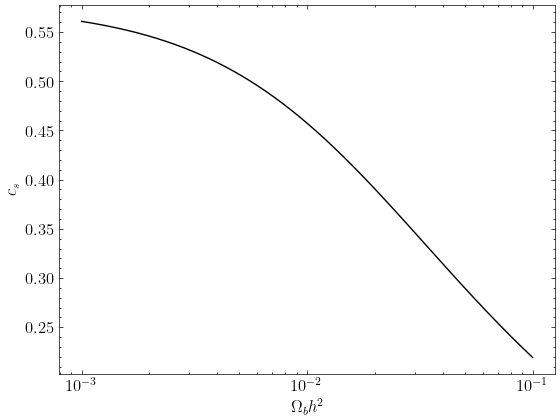
\includegraphics[width=0.6\textwidth]{speed_of_sound}
        \caption{Vitesse du son lors du découplement (fraction de la 
        vitesse de la lumière).}
        \label{fig:spped_of_sound}
\end{figure}

\subsection{Nombre d'onde de Jeans}
Le nombre d'onde de Jeans dans les coordonnées comobiles est 
\[
        k_J = \sqrt{\frac{4\pi G \rho_b a^2}{c_s^2}}
\]
et décrit la taille minimale d'un objet de densité de matière $\rho_b$ 
pour l'instabilité de Jeans (effondrement gravitationnel). 
On s'intéresse à la période avant le découplement, donc 
$a < a_{\text{dec}}$. À ce moment, l'Univers est dominé par 
la radiation donc ($a(t=0) = 0$):
\[
        \dot{a} = H_0 \Omega_r^{1/2}a^{-1} \implies 
        a(t) = \left( 2H_0\Omega_r^{1/2} t \right)^{1/2}
\]
Donc, l'horizon est
\[
        \eta(t) = \int_{0}^{t} \frac{dt'}{a(t')} 
        = \sqrt{\frac{t}{2H_0\Omega_r^{1/2}}} = \frac{a}{2H_0 \Omega_r^{1/2}}
\]
Malgré le fait que $k_J$ diminue en fonction de $a$, l'accélération 
de l'expansion de l'Univers fait en sorte que $\eta k_J \rightarrow 1$ 
environ au moment du découplement, ce qui permet au large structure de 
l'Univers de commencer à se former sous l'attraction gravitationnelle.
\begin{figure}[H]
        \centering
        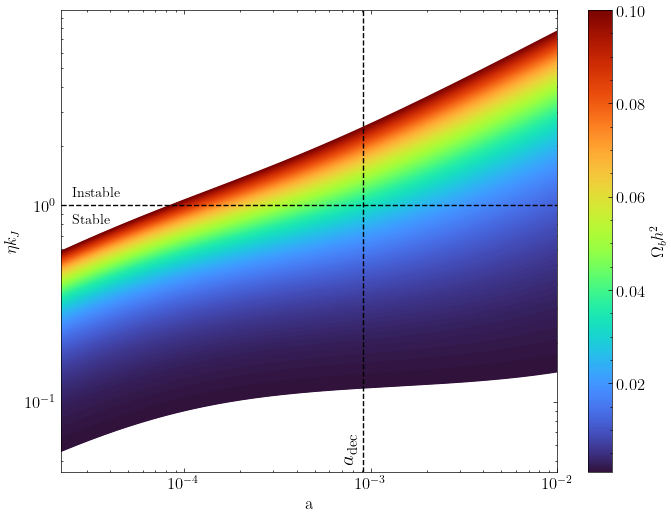
\includegraphics[width=0.8\textwidth]{eta_kj}
        \caption{Rapport de la longueur d'onde de Jeans et de l'horizon cosmique. 
        Lorsque $\eta k_J < 1$, la matière est stable par rapport au instabilités gravitationnelles. On 
remarque que $\eta k_J < 1$ pour $a < a_{\text{dec}}$ et $\Omega_b h^2 \lesssim 0.022$ 
ce qui correspond bien à un Univers stable avant 
le découplement.}
\end{figure}


\section{La vraisemblance}
On considère la fonction de vraisemblance Gaussienne:
\[
        \mathcal{L}(\mathcal{D} \mid w, \sigma_w^2) 
        = \frac{1}{(2 \pi \sigma_w^2)^{|\mathcal{D}|/2}}
        \exp \left\{ -\sum_{i=1}^{|\mathcal{D}|}\frac{(d_i - w)^{2} }{2 \sigma_w^2} \right\}
\]
où $\mathcal{D} = \{d_i \}$ est le jeu de données et $|\mathcal{D}|$ est 
la taille du jeu de donnée.
On cherche l'erreur sur la déviation standard $\sigma_w$. On suppose que la 
fonction de vraisemblance est quadratique autour de la solution MLE. 
\[
        \ln \mathcal{L}(\mathcal{\mathcal{D}} \mid \sigma_w, w=\bar{w}) \simeq 
        \ln \mathcal{L}(\mathcal{D} \mid \bar{\sigma}_w, \bar{w}) 
        + \frac{1}{2}\frac{\partial^2 \ln \mathcal{L}}{\partial \sigma_w^2} 
        \bigg|_{\sigma_w=\bar{\sigma}_w} (\sigma_w - \bar{\sigma}_w)^{2}
\]
En effet, on sait que
\[
        \frac{\partial \ln \mathcal{L}}{\partial \sigma_w}\bigg|_{\text{MLE}} = 
        \frac{1}{\bar{\sigma}_w^{3}}\sum_{i=1}^{|\mathcal{D}|}(d_i - \bar{w})^{2} - 
        \frac{|\mathcal{D}|}{\bar{\sigma}_w} = 0
\]
D'où on avait trouvé la solution MLE pour la variance
\[
        \bar{\sigma}^2_w = 
        \frac{1}{|\mathcal{D}|}\sum_{i=1}^{|\mathcal{D}|}(d_i - \bar{w})^{2}
\]
Où $\bar{w}$ est la solution attendu pour le signal $w$ (moyenne). L'erreur 
sur la déviation standard est 2 fois l'inverse du 
coefficient de deuxième ordre dans 
l'expansion de Taylor de la vraisemblance autour de son maximum global (
définition de FHWM):
\begingroup
\allowdisplaybreaks
\begin{align*}
        \sigma_{\sigma_w}^{-1} &= -\frac{\partial^2 \ln \mathcal{L}}{\partial \sigma_w^2}
        \bigg|_{\text{MLE}} \\
                          &= \frac{3}{\bar{\sigma}_w^4}\sum_{i=1}^{|\mathcal{D}|}
        (d_i - \bar{w})^{2} - \frac{|\mathcal{D}|}{\bar{\sigma}_w^{2}} \\
                          &= \frac{2|\mathcal{D}|^2}{
                          \displaystyle \sum_{i=1}^{|\mathcal{D}|}(d_i - \bar{w})^{2}} \\
        \implies \Aboxed{  \sigma_{\sigma_w}  &= \frac{1}{2|\mathcal{D}|^{2}}
        \sum_{i = 1}^{|\mathcal{D}|}(d_i -\bar{w})^{2} = \frac{\bar{\sigma}_w}{2|\mathcal{D}|}}
\end{align*}
\endgroup
Donc l'incertitude sur la déviation standard diminue très rapidement 
avec la taille du jeu de donnée $|\mathcal{D}|$.




%La valeur de $a_{\text{rec}}$ (et particulièrement de $z_{\text{rec}}$) 
%est très sensible à $X_e$. En principe, on doit résoudre l'équation de 
%Boltzmann pour le processus de recombinaison pour déterminer sa valeur. 
%où $\text{Ry} = 2 \pi \hbar c R_{\infty } = m_e + m_p - m_h$ 
%est la constante de Rydberg. Avec $n_h = n_b(1 - X_e)$ on 
%obtient
%\[
        %a^{-3} \frac{d(n_e a^3)}{dt} =  (1 - X_e)n_b\beta  - X_e^2n_b^2\alpha^{(2)}
%\]
%où $\beta$ est le taux d'ionisation (on réintroduit les unités physiques)
%\[
        %\beta \equiv 
        %\alpha^{(2)} c\left( \frac{m_e k_B T}{2 \pi \hbar^{2}} \right)^{3/2}
        %\exp \left\{ -\frac{\text{Ry}}{k_B T} \right\}
%\]
%et $\alpha^{(2)} = \expval{\sigma v}$ est la section efficace thermalisée 
%excluant 
%le niveau fondamental $n = 1$ puisque le photon de recombinaison
%de cet état état va ioniser immédiatement un atome $H$ voisin. 
%On omet le détail de ce calcul et on se réfère à l'équation (3.42)
%de Dodelson pour une approximation de cette section efficace
%\[
        %\alpha^{(2)} = 9.78 \frac{\hbar^2\alpha^{2}}{m_e^2c^2} 
        %\left( \frac{\text{Ry}}{k_BT}  \right)^{1/2}
        %\ln \left( \frac{\text{Ry}}{k_BT} \right)
%\]
%Sachant qu'au moment de la recombinaison, la température de la 
%matière est approximativement la même que la température des 
%photons à cause des processus de diffusion, on a
%\[
        %T = T_{\text{CMB}}a^{-1} = 2.725\,48\, a^{-1}\,\,\text{K}
%\]
%On a donc des expressions en terme du facteur d'échelle pour 
%la plupart des quantités d'intérêt. On revient à l'équation de 
%Boltzmann pour changer la variable d'intégration et simplifier le 
%côté gauche. En effet, on réalise que $n_e a^3 \simeq X_e n_b a^3$. 
%D'où
%\[
        %\frac{dX_e}{dt} =  (1 - X_e(a))\beta(a)  - X_e^2(a)n_b\alpha^{(2)}(a)
%\]
%On utilise la seconde équation de Friedmann pour une expression 
%de $dt$ dans le régime matière-radiation qui nous intéresse:
%\[
        %dt = \frac{da}{H_0 \sqrt{\Omega_0 a^{-2} + \Omega_m a^{-1}}}
%\]
%d'où l'équation différentielle
%\[
        %\frac{dX_e}{da} = (100\, \text{km}\,\text{s}^{-1}\, \text{Mpc}^{-1})^{-1}
        %\frac{ (1 - X_e(a))\beta(a)  - X_e^2(a)n_b\alpha^{(2)}(a)}{
        %h\sqrt{\Omega_r a^{-2} + \Omega_m a^{-1}}}
%\]



\end{document}

